\chapter{Referencial Teórico}
\label{cap:referencial-reorico}

\section{O que é Machine Learning?}
\label{sec:oqueemachinelearning}

Não existe uma definição que seja aceita por todos, porem o principal objetivo de ML é identificar padrões e realizar ações, oque remete ao aprendizado,
que em sua base é identificar padrões e saber reconhece-los quando vê-los novamente. O processo básico de aprendizagem consiste em entrada de dados, abstração e generalização.
\begin{alineas}
	\item Entrada de dados: são fatos tirados da memoria ou da observação;
	\item Abstração: transformar estes dados em algo mais objetivo e que faça sentido;
	\item Generalização: utiliza os dados abstraídos e para  identificar padrões e assim classifica-los;			
\end{alineas}

\begin{figure}[h!]
	\centering
	\Caption{\label{fig:processo-aprendizagem} Fluxo do processo de aprendizagem.}	
	\UECEfig{}{
		\fbox{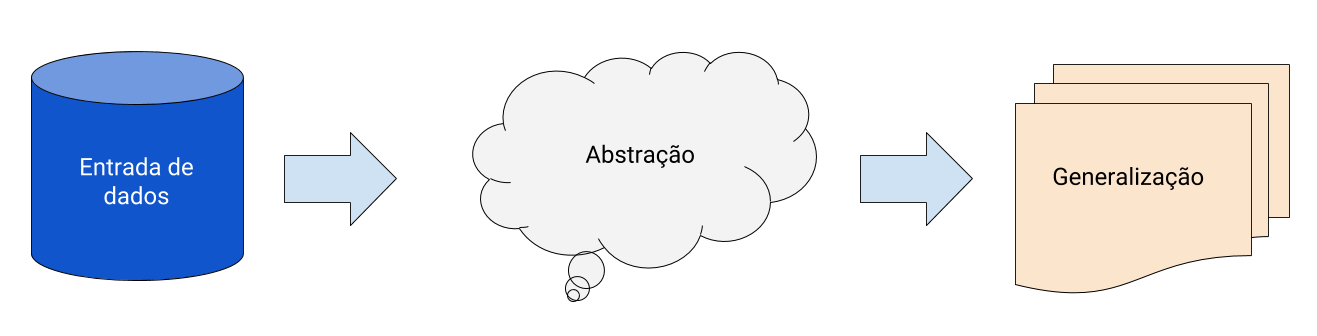
\includegraphics[width=15cm]{figuras/procc-learning}}
	}{
		\Fonte{Elaborado pelo autor}
	}	
\end{figure}

Todo este processo ocorre na ordem apresentada, pois o conceito de abstração e generalização estão muito próximos e tecnicamente um não faz sentido sem o outro. Os passos de abstração e generalização do processo de aprendizagem ocorrem subconscientemente em seres humanos, logo pode ser complexo representar este processo em linguagem computacional.


\subsection{Abstração e Representação de Dados}
\label{cap:abs-representacao-dados}

Durante a abstração os dados de entradas, são preparados para que possuam algum sentido em um contexto. Para ilustrar este processo, lembre de quando aprendeu a executar operações de soma e subtração, que sua professora apresentou o seguinte exemplo:
Uma maçã mais outra maçã é igual à duas maçãs, você deixou de lado todas as propriedades da maçã como ser uma fruta, ter a cor vermelha  ou possuir sementes, para um tipo de unidade , uma unidade de um tipo mais outra unidade do mesmo tipo é igual à duas unidades, ou seja para o contexto de soma não importa se é uma fruta ou a cor e sim a unidade.